\documentclass[12 pt]{extarticle}

	\usepackage[frenchb]{babel}
	\usepackage[utf8]{inputenc}  
	\usepackage[T1]{fontenc}
	\usepackage{amssymb}
	\usepackage[mathscr]{euscript}
	\usepackage{stmaryrd}
	\usepackage{amsmath}
	\usepackage{tikz}
	\usepackage[all,cmtip]{xy}
	\usepackage{amsthm}
	\usepackage{varioref}
	\usepackage{geometry}
	\geometry{a4paper}
	\usepackage{lmodern}
	\usepackage{hyperref}
	\usepackage{array}
	 \usepackage{fancyhdr}
\renewcommand{\theenumi}{\alph{enumi})}
	\pagestyle{fancy}
	\theoremstyle{plain}
	\fancyfoot[C]{} 
	\fancyhead[L]{Fiche d'exercices}
	\fancyhead[R]{2023-2024}\geometry{
 a4paper,
 total={170mm,257mm},
 left=20mm,
 top=20mm,
 }
	
	
	\title{Exercices Chapitre 8}
	\date{}
	\begin{document}

\begin{center}{\Large Chapitre 8 - Aires}\\ 
 \end{center}
 
  \subsection*{Exercices mentaux - manuel primaire 1896}
  
\begin{enumerate}
\item Combien y a-t-il de mètres carrés dans un décamètre carré ? dans un hectomètre carré ? dans $4$ décamètres carrés ? dans $6$ hectomètres carrés ? 
\item Combien font de mètres carrés : 4 décamètres carrés ? 9 décamètres carrés ? 42 décamètres carrés ? 
2 hectomètres carrés ? 7 hectomètres carrés ? 24 décamètres carrés ? 9 hectomètres carrés ? 
\item Combien dans un mètre carré y a-t-il : de décimètres carrés ? de centimètres carrés ? de millimètres carrés ? 
\item Combien faut-il de décimètres carrés pour faire : 3 mètres carrés ? 8 mètres carrés ? 35 mètres carrés ? 
\item Combien faut-il de centimètres carrés pour faire : 6 mètres carrés ? 12 mètres carrés ? 63 mètres carrés ? 
\item Combien l'hectomètre carré vaut-il : de décamètres carrés ? de mètres carrés ? de décimètres carrés ? 
\item Combien le décamètre carré vaut-il : de mètres carrés ? de décimètres carrés ? de centimètres carrés ? 
\item Combien le décimètre carré vaut-il de centimètres carrés ?
\item Quelle est l'unité de mesure de surface $100$ fois plus grande que le mètre carré ? que le décamètre carré ? que le décimètre carré ? que le centimètre carré ?
\item Quelle est l'unité de mesure de surface
$10~000$ fois plus grande que le mètre carré ? que le centimètre carré ? que le décimètre carré ? 
\item Quelle est l'unité de mesure de surface $100$ fois plus petite que l'hectomètre carré ? que le décamètre carré ? que le décimètre carré ? que le mètre carré ? 
\item Quelle est l'unité de mesure de surface : 10~000 fois plus petite que l'hectomètre carré ? 10~000 fois plus grande que le décimètre carré ? 
\item Quelle est l'unité de mesure de surface : 100 fois plus grande que le centimètre carré ? 100 fois plus petite que le décimètre carré ? 10~000 fois plus grande que le mètre carré ? 10~000 fois plus petite que le décamètre carré ? 
\item Quels sont les deux rangs à gauche de la virgule occupés par les mètres carrés ? par les hectomètres carrés ? par les décamètres carrés ? 
\item Quels sont les deux rangs à droite de la virgule
occupés par les décimètres carrés ? par les centimètres carrés ? 
\item Quels sont les rangs à droite et à gauche de la virgule occupés par les décamètres carrés ? par les décimètres carrés ? par les centimètres carrés ? par les mètres carrés ? 
\end{enumerate}  
  
  
  \subsection*{Exercices d'applications - manuel primaire 1896}
  
  \begin{enumerate}
  \item On possède deux champs, l'un de $65$ décamètres carrés, l'autre de $34$ ares. 
  Quelle est leur étendue totale ? 
  \item L'étendue totale de deux terrains est de $3$ hectares $4$ ares. Le premier a $40$ ares. Quelle est l'étendue du second ? 
  \item Un terrain a une surface de $2$ hectares $14$ ares. Il a été payé $25$ centimes le mètre carré. Quel en est le prix ? 
  \item Quel est le prix d'un terrain de $3$ hectares, $14$ ares, $6$ centiares à raison de $24$ euros $50$ le décamètre carré. 
  \item Si on ajoutait $345$ mètres carrés à l'étendue d'un champ, on aurait une surface de $6$ ares. Quelle est cette étendue ? 
  \item Quel est le prix d'un hectare de terre, lorsque le mètre carré coûte $0,2835$ euros ? 
  \item Un champ de $4$ hectares $5$ ares a été partagé entre $3$ personnes. La première doit avoir $350$ mètres carrés de plus que la deuxième. Celle-ci a $3~500$ mètres carrés. Quelle sera la part de la troisième ? 
  \item Quelle est la surface d'un rectangle de $90$ mètres de long sur $75$ mètres de large ? 
  \item Deux champs ont la même superficie. L'un vaut $26$ euros $50$ l'are, l'autre $3~500$ euros l'hectare. Quelle est la différence des prix, cette superficie étant de $4$ hectares ? 
  \item Un terrain a une forme rectangulaire de $125$ mètres de long sur $110$ de large. Quelle est sa surface ? 
  \end{enumerate}


\subsection*{Exercices à base de formules}
Calculez les aires des surfaces suivantes, en mètres carrés, puis en hectares.
\begin{enumerate}
\item Une salle rectangulaire de 12 m sur 20 m.
\item Un champ rectangulaire de 120 m sur 85 m
\item Un parc rectangulaire de 843 m sur 12 dam. 
\item Un mur rectangulaire de 2 m sur 9 m. 
\item Une place carrée de 65 m de côté. 
\item Un pâté de maison en forme de triangle rectangle de $5$ hm sur $43$ dam. 
\item Un triangle dont la base mesure $234$ cm et la hauteur $12$ m. 
\item Une salle en forme de disque de rayon $9,4$ m. 
\item Une salle en forme de disque de diamètre $3,5$ dam. 
\
\end{enumerate}


\subsection*{Figures composées}

Sur toutes les figures suivantes, on considère que les carreaux ont 1 centimètre de côté. Calculez les aires des figures suivantes, en donnant d'abord une valeur exacte, puis une valeur approchée au millimètre carré s'il y a lieu. 
\[ 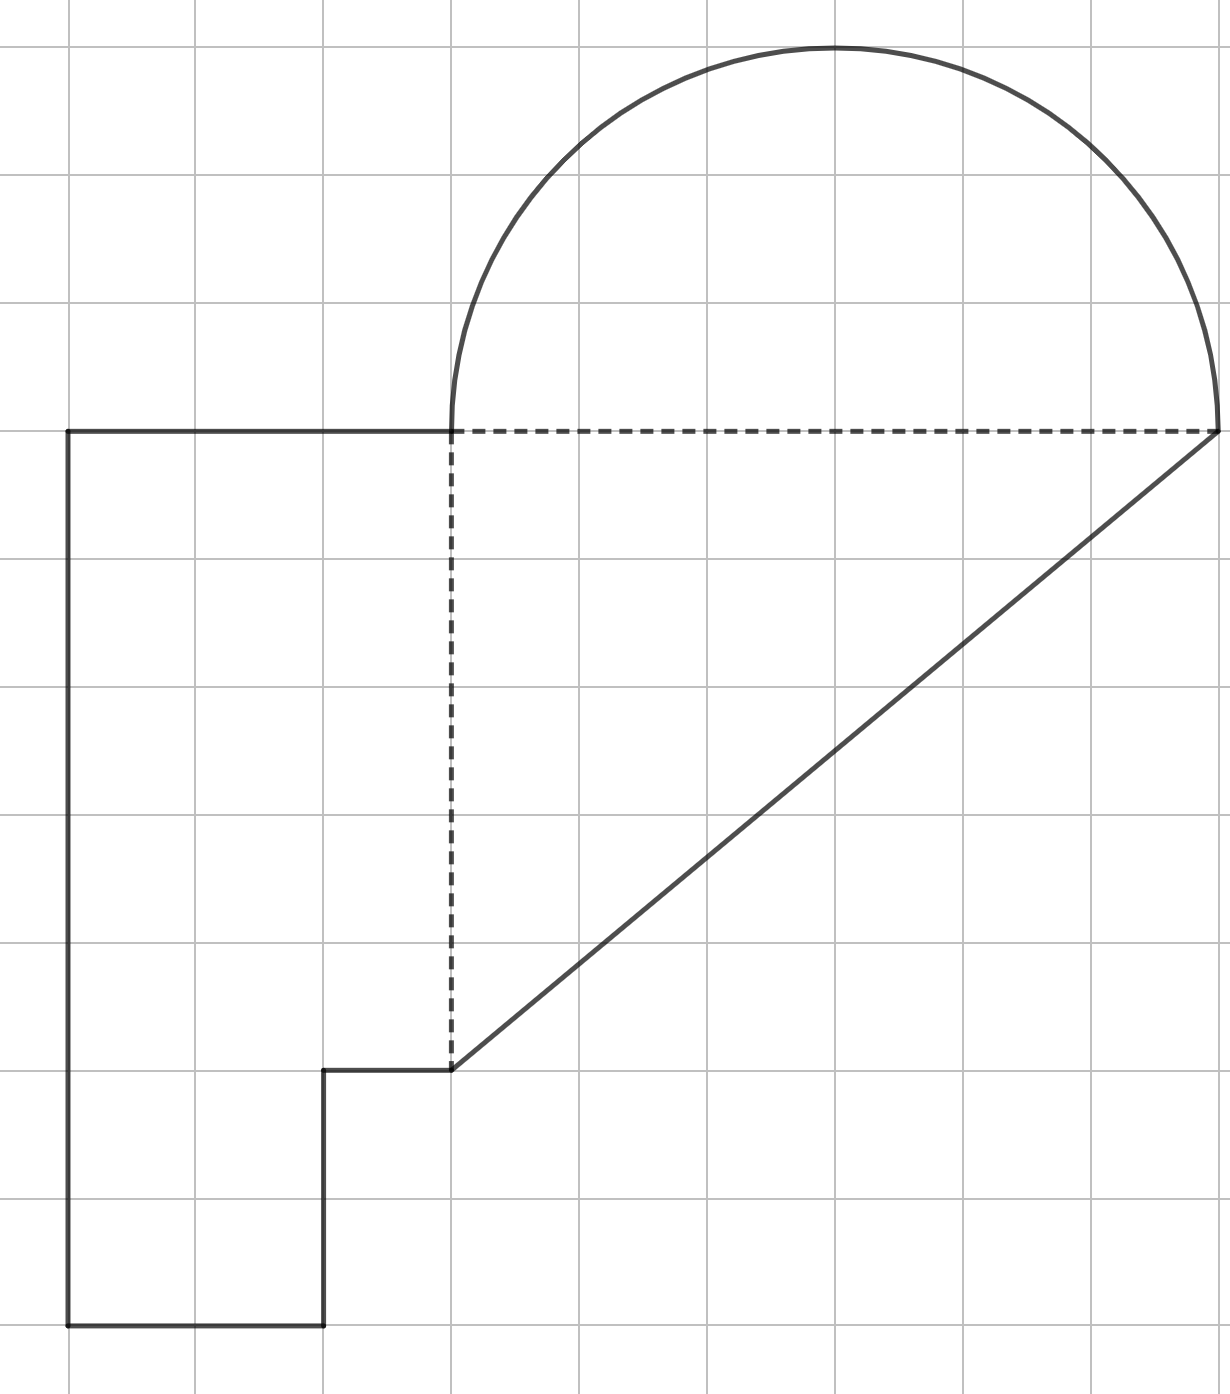
\includegraphics[scale=.3]{Fig1}\ \ 
\ 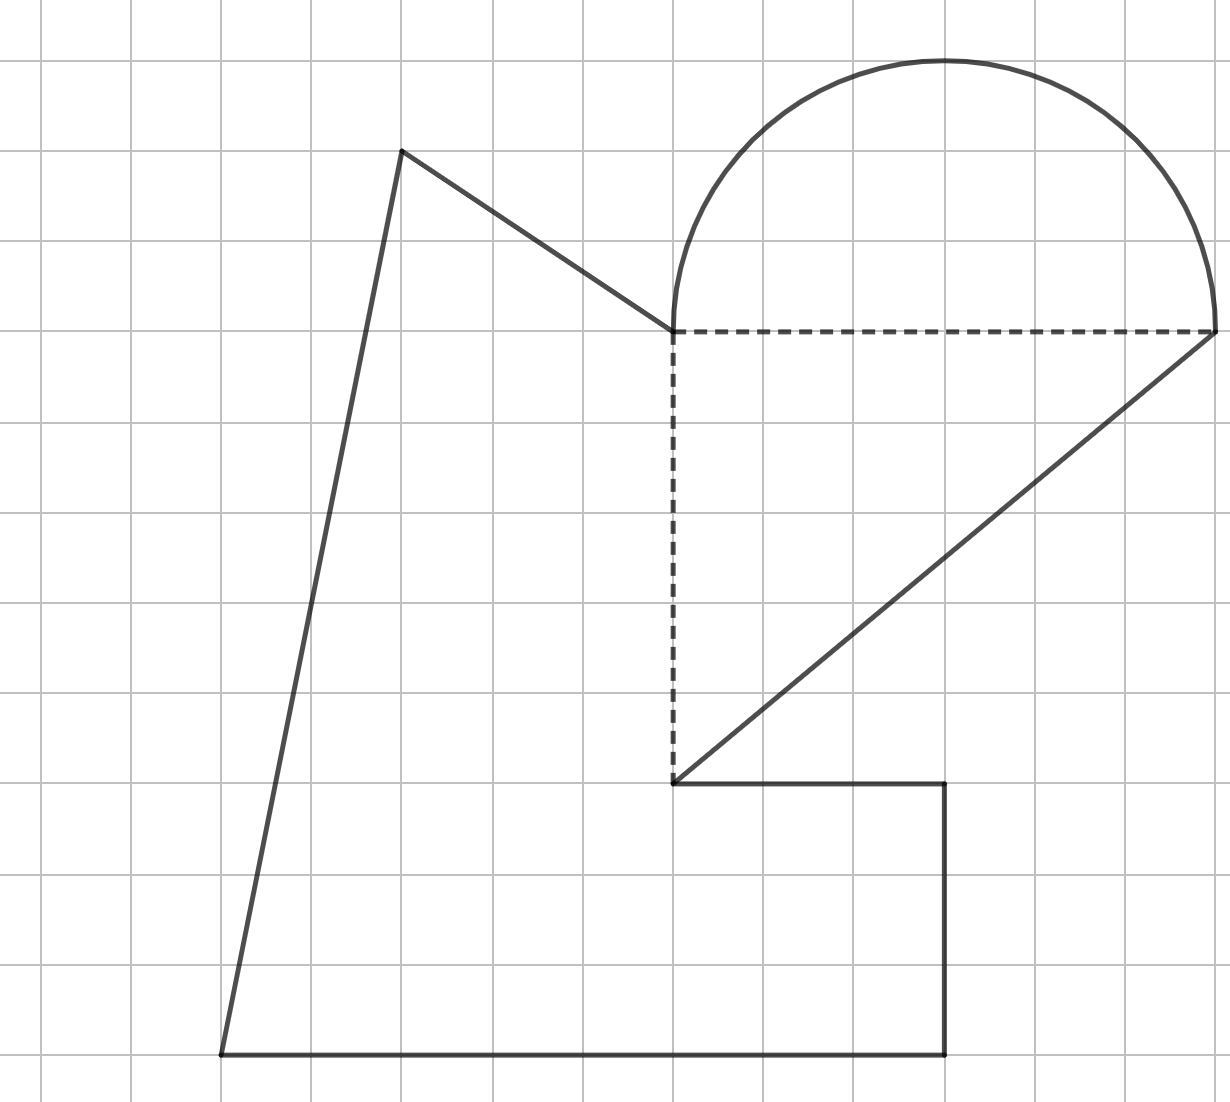
\includegraphics[scale=.4]{Fig2} \]


\[ 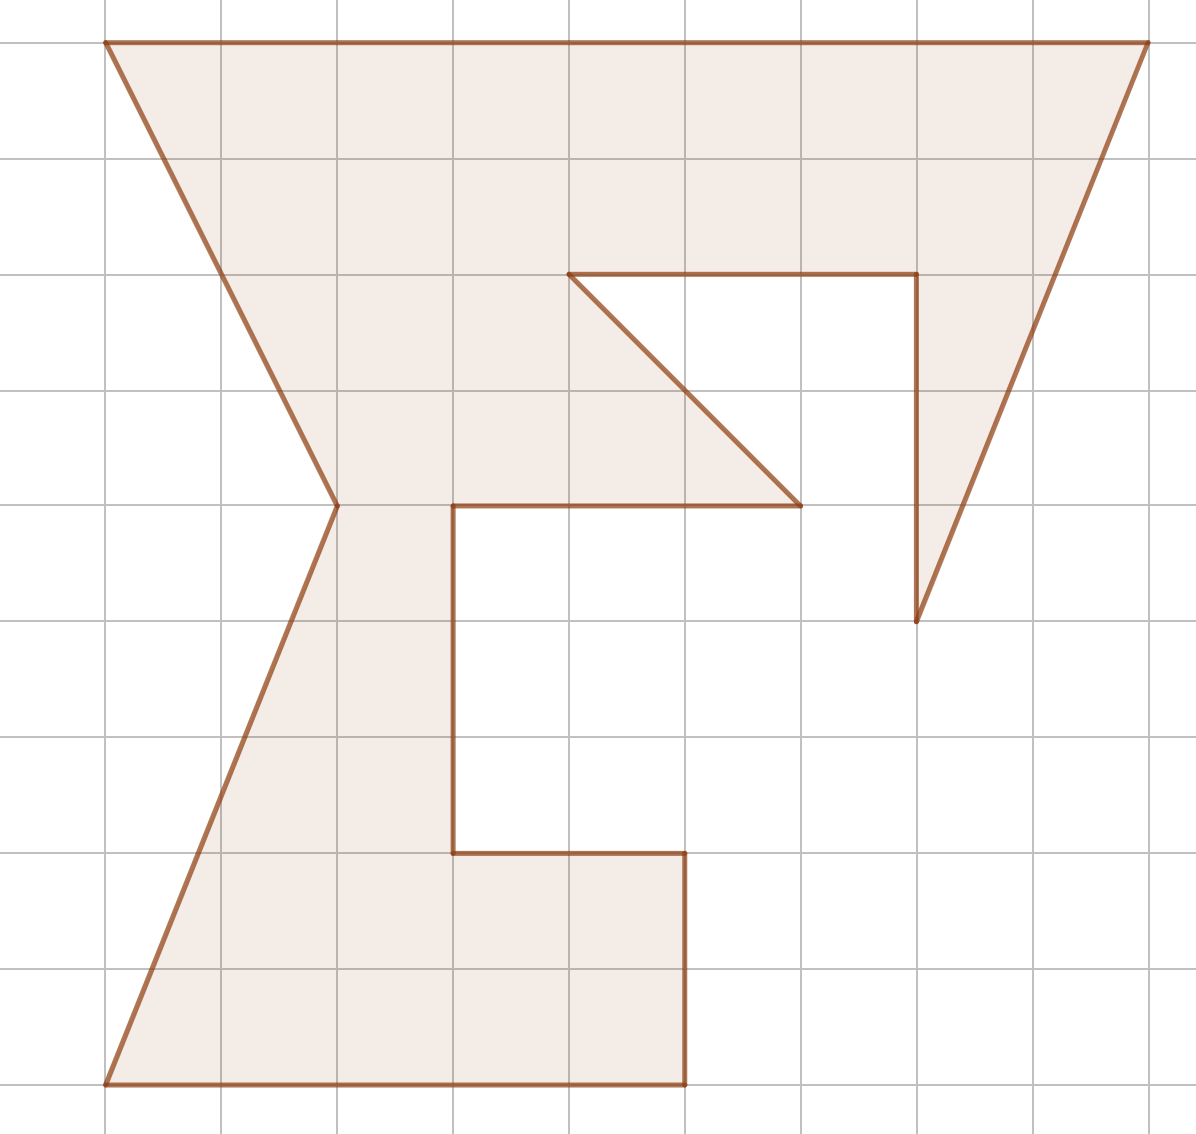
\includegraphics[scale=.4]{Fig3}\ \ 
\ 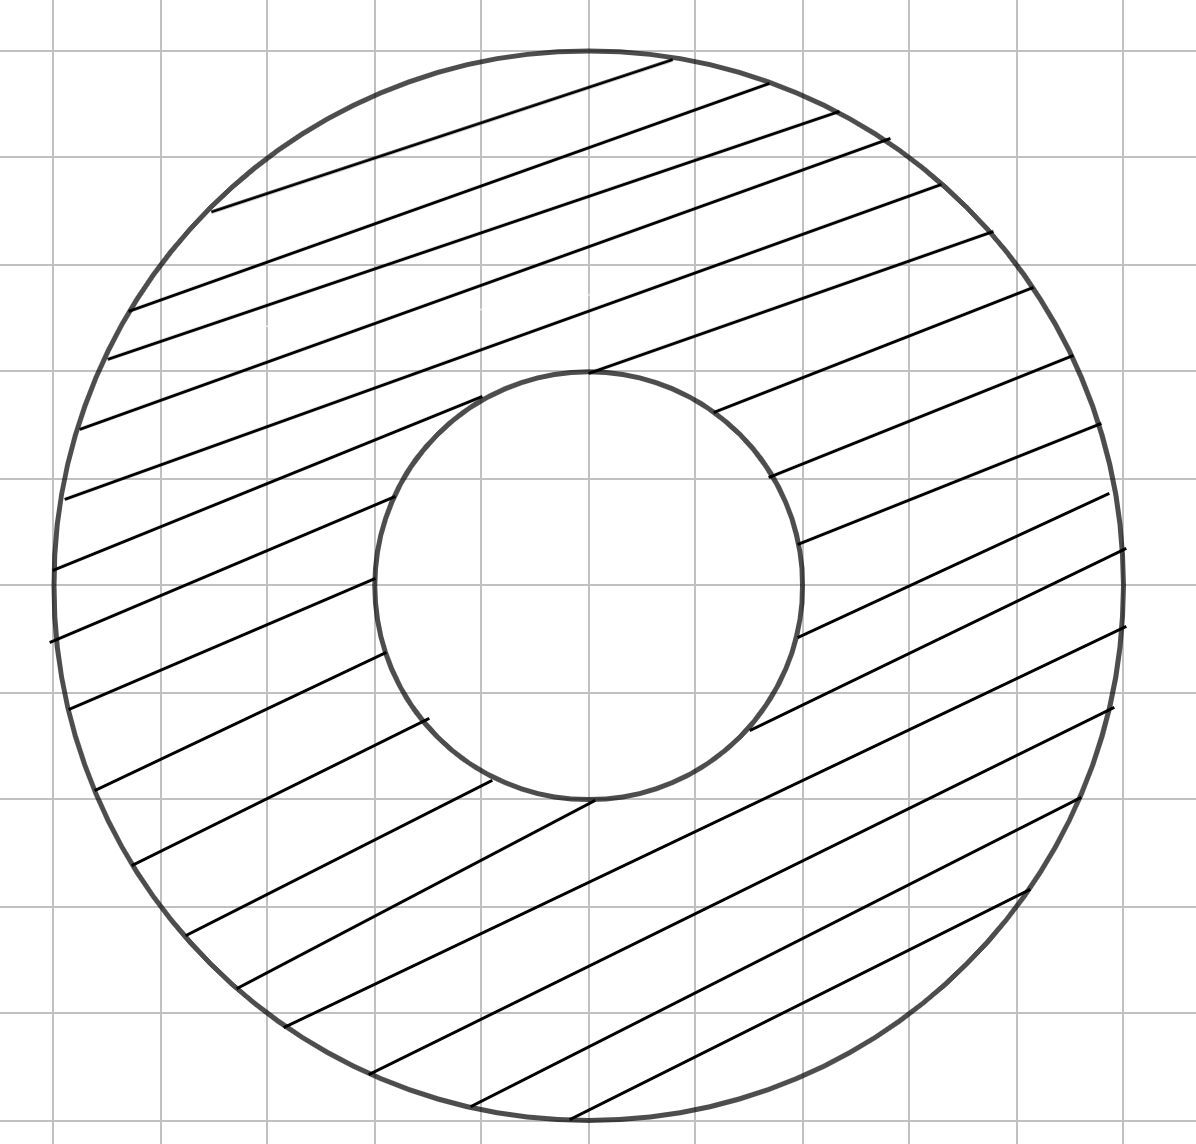
\includegraphics[scale=.4]{Fig4} \]

\[ 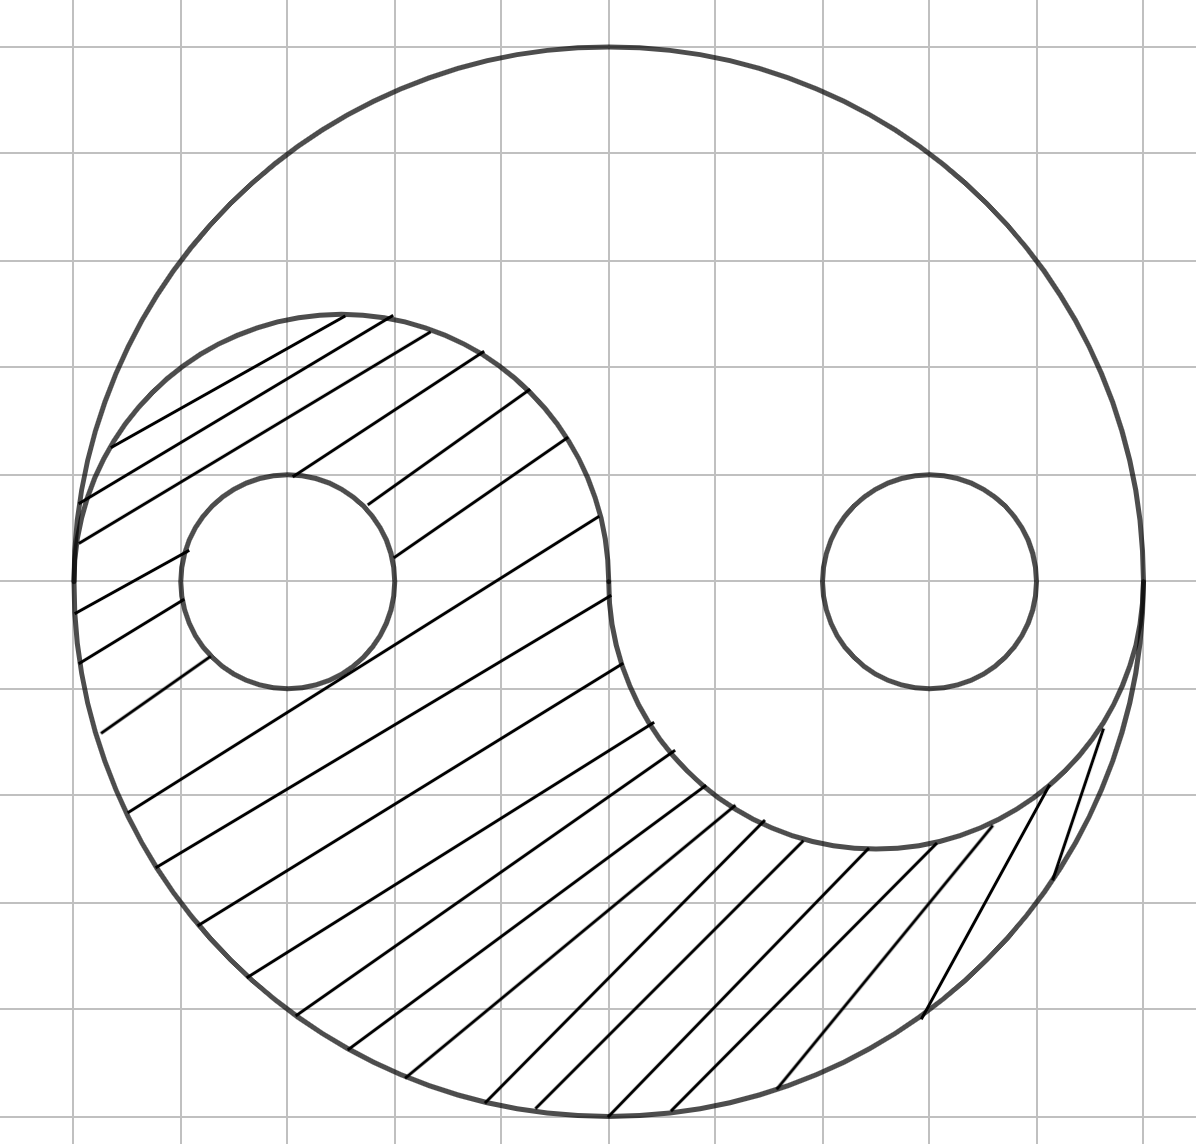
\includegraphics[scale=.4]{Fig5} \]
 	\end{document}
